\documentclass[12pt]{article}
%Fall 2022
% Some basic packages
\usepackage{standalone}[subpreambles=true]
\usepackage[utf8]{inputenc}
\usepackage[T1]{fontenc}
\usepackage{textcomp}
\usepackage[english]{babel}
\usepackage{url}
\usepackage{graphicx}
%\usepackage{quiver}
\usepackage{float}
\usepackage{enumitem}
\usepackage{lmodern}
\usepackage{comment}
\usepackage{hyperref}
\usepackage[usenames,svgnames,dvipsnames]{xcolor}
\usepackage[margin=1in]{geometry}
\usepackage{pdfpages}

\pdfminorversion=7

% Don't indent paragraphs, leave some space between them
\usepackage{parskip}

% Hide page number when page is empty
\usepackage{emptypage}
\usepackage{subcaption}
\usepackage{multicol}
\usepackage[b]{esvect}

% Math stuff
\usepackage{amsmath, amsfonts, mathtools, amsthm, amssymb}
\usepackage{bbm}
\usepackage{stmaryrd}
\allowdisplaybreaks

% Fancy script capitals
\usepackage{mathrsfs}
\usepackage{cancel}
% Bold math
\usepackage{bm}
% Some shortcuts
\newcommand{\rr}{\ensuremath{\mathbb{R}}}
\newcommand{\zz}{\ensuremath{\mathbb{Z}}}
\newcommand{\qq}{\ensuremath{\mathbb{Q}}}
\newcommand{\nn}{\ensuremath{\mathbb{N}}}
\newcommand{\ff}{\ensuremath{\mathbb{F}}}
\newcommand{\cc}{\ensuremath{\mathbb{C}}}
\newcommand{\ee}{\ensuremath{\mathbb{E}}}
\newcommand{\hh}{\ensuremath{\mathbb{H}}}
\renewcommand\O{\ensuremath{\emptyset}}
\newcommand{\norm}[1]{{\left\lVert{#1}\right\rVert}}
\newcommand{\dbracket}[1]{{\left\llbracket{#1}\right\rrbracket}}
\newcommand{\ve}[1]{{\bm{#1}}}
\newcommand\allbold[1]{{\boldmath\textbf{#1}}}
\DeclareMathOperator{\lcm}{lcm}
\DeclareMathOperator{\im}{im}
\DeclareMathOperator{\coim}{coim}
\DeclareMathOperator{\dom}{dom}
\DeclareMathOperator{\tr}{tr}
\DeclareMathOperator{\rank}{rank}
\DeclareMathOperator*{\var}{Var}
\DeclareMathOperator*{\ev}{E}
\DeclareMathOperator{\dg}{deg}
\DeclareMathOperator{\aff}{aff}
\DeclareMathOperator{\conv}{conv}
\DeclareMathOperator{\inte}{int}
\DeclareMathOperator*{\argmin}{argmin}
\DeclareMathOperator*{\argmax}{argmax}
\DeclareMathOperator{\graph}{graph}
\DeclareMathOperator{\sgn}{sgn}
\DeclareMathOperator*{\Rep}{Rep}
\DeclareMathOperator{\Proj}{Proj}
\DeclareMathOperator{\mat}{mat}
\DeclareMathOperator{\diag}{diag}
\DeclareMathOperator{\aut}{Aut}
\DeclareMathOperator{\gal}{Gal}
\DeclareMathOperator{\inn}{Inn}
\DeclareMathOperator{\edm}{End}
\DeclareMathOperator{\Hom}{Hom}
\DeclareMathOperator{\ext}{Ext}
\DeclareMathOperator{\tor}{Tor}
\DeclareMathOperator{\Span}{Span}
\DeclareMathOperator{\Stab}{Stab}
\DeclareMathOperator{\cont}{cont}
\DeclareMathOperator{\Ann}{Ann}
\DeclareMathOperator{\Div}{div}
\DeclareMathOperator{\curl}{curl}
\DeclareMathOperator{\nat}{Nat}
\DeclareMathOperator{\gr}{Gr}
\DeclareMathOperator{\vect}{Vect}
\DeclareMathOperator{\id}{id}
\DeclareMathOperator{\Mod}{Mod}
\DeclareMathOperator{\sign}{sign}
\DeclareMathOperator{\Surf}{Surf}
\DeclareMathOperator{\fcone}{fcone}
\DeclareMathOperator{\Rot}{Rot}
\DeclareMathOperator{\grad}{grad}
\DeclareMathOperator{\atan2}{atan2}
\DeclareMathOperator{\Ric}{Ric}
\let\vec\relax
\DeclareMathOperator{\vec}{vec}
\let\Re\relax
\DeclareMathOperator{\Re}{Re}
\let\Im\relax
\DeclareMathOperator{\Im}{Im}
% Put x \to \infty below \lim
\let\svlim\lim\def\lim{\svlim\limits}

%wide hat
\usepackage{scalerel,stackengine}
\stackMath
\newcommand*\wh[1]{%
\savestack{\tmpbox}{\stretchto{%
  \scaleto{%
    \scalerel*[\widthof{\ensuremath{#1}}]{\kern-.6pt\bigwedge\kern-.6pt}%
    {\rule[-\textheight/2]{1ex}{\textheight}}%WIDTH-LIMITED BIG WEDGE
  }{\textheight}% 
}{0.5ex}}%
\stackon[1pt]{#1}{\tmpbox}%
}
\parskip 1ex

%Make implies and impliedby shorter
\let\implies\Rightarrow
\let\impliedby\Leftarrow
\let\iff\Leftrightarrow
\let\epsilon\varepsilon

% Add \contra symbol to denote contradiction
\usepackage{stmaryrd} % for \lightning
\newcommand\contra{\scalebox{1.5}{$\lightning$}}

% \let\phi\varphi

% Command for short corrections
% Usage: 1+1=\correct{3}{2}

\definecolor{correct}{HTML}{009900}
\newcommand\correct[2]{\ensuremath{\:}{\color{red}{#1}}\ensuremath{\to }{\color{correct}{#2}}\ensuremath{\:}}
\newcommand\green[1]{{\color{correct}{#1}}}

% horizontal rule
\newcommand\hr{
    \noindent\rule[0.5ex]{\linewidth}{0.5pt}
}

% hide parts
\newcommand\hide[1]{}

% si unitx
\usepackage{siunitx}
\sisetup{locale = FR}

%allows pmatrix to stretch
\makeatletter
\renewcommand*\env@matrix[1][\arraystretch]{%
  \edef\arraystretch{#1}%
  \hskip -\arraycolsep
  \let\@ifnextchar\new@ifnextchar
  \array{*\c@MaxMatrixCols c}}
\makeatother

\renewcommand{\arraystretch}{0.8}

\renewcommand{\baselinestretch}{1.5}

\usepackage{graphics}
\usepackage{epstopdf}

\RequirePackage{hyperref}
%%
%% Add support for color in order to color the hyperlinks.
%% 
\hypersetup{
  colorlinks = true,
  urlcolor = blue,
  citecolor = blue
}
%%fakesection Links
\hypersetup{
    colorlinks,
    linkcolor={red!50!black},
    citecolor={green!50!black},
    urlcolor={blue!80!black}
}
%customization of cleveref
\RequirePackage[capitalize,nameinlink]{cleveref}[0.19]

% Per SIAM Style Manual, "section" should be lowercase
\crefname{section}{section}{sections}
\crefname{subsection}{subsection}{subsections}
\Crefname{section}{Section}{Sections}
\Crefname{subsection}{Subsection}{Subsections}

% Per SIAM Style Manual, "Figure" should be spelled out in references
\Crefname{figure}{Figure}{Figures}

% Per SIAM Style Manual, don't say equation in front on an equation.
\crefformat{equation}{\textup{#2(#1)#3}}
\crefrangeformat{equation}{\textup{#3(#1)#4--#5(#2)#6}}
\crefmultiformat{equation}{\textup{#2(#1)#3}}{ and \textup{#2(#1)#3}}
{, \textup{#2(#1)#3}}{, and \textup{#2(#1)#3}}
\crefrangemultiformat{equation}{\textup{#3(#1)#4--#5(#2)#6}}%
{ and \textup{#3(#1)#4--#5(#2)#6}}{, \textup{#3(#1)#4--#5(#2)#6}}{, and \textup{#3(#1)#4--#5(#2)#6}}

% But spell it out at the beginning of a sentence.
\Crefformat{equation}{#2Equation~\textup{(#1)}#3}
\Crefrangeformat{equation}{Equations~\textup{#3(#1)#4--#5(#2)#6}}
\Crefmultiformat{equation}{Equations~\textup{#2(#1)#3}}{ and \textup{#2(#1)#3}}
{, \textup{#2(#1)#3}}{, and \textup{#2(#1)#3}}
\Crefrangemultiformat{equation}{Equations~\textup{#3(#1)#4--#5(#2)#6}}%
{ and \textup{#3(#1)#4--#5(#2)#6}}{, \textup{#3(#1)#4--#5(#2)#6}}{, and \textup{#3(#1)#4--#5(#2)#6}}

% Make number non-italic in any environment.
\crefdefaultlabelformat{#2\textup{#1}#3}

% Environments
\makeatother
% For box around Definition, Theorem, \ldots
%%fakesection Theorems
\usepackage{thmtools}
\usepackage[framemethod=TikZ]{mdframed}

\theoremstyle{definition}
\mdfdefinestyle{mdbluebox}{%
	roundcorner = 10pt,
	linewidth=1pt,
	skipabove=12pt,
	innerbottommargin=9pt,
	skipbelow=2pt,
	nobreak=true,
	linecolor=blue,
	backgroundcolor=TealBlue!5,
}
\declaretheoremstyle[
	headfont=\sffamily\bfseries\color{MidnightBlue},
	mdframed={style=mdbluebox},
	headpunct={\\[3pt]},
	postheadspace={0pt}
]{thmbluebox}

\mdfdefinestyle{mdredbox}{%
	linewidth=0.5pt,
	skipabove=12pt,
	frametitleaboveskip=5pt,
	frametitlebelowskip=0pt,
	skipbelow=2pt,
	frametitlefont=\bfseries,
	innertopmargin=4pt,
	innerbottommargin=8pt,
	nobreak=false,
	linecolor=RawSienna,
	backgroundcolor=Salmon!5,
}
\declaretheoremstyle[
	headfont=\bfseries\color{RawSienna},
	mdframed={style=mdredbox},
	headpunct={\\[3pt]},
	postheadspace={0pt},
]{thmredbox}

\declaretheorem[%
style=thmbluebox,name=Theorem,numberwithin=section]{thm}
\declaretheorem[style=thmbluebox,name=Lemma,sibling=thm]{lem}
\declaretheorem[style=thmbluebox,name=Proposition,sibling=thm]{prop}
\declaretheorem[style=thmbluebox,name=Corollary,sibling=thm]{coro}
\declaretheorem[style=thmredbox,name=Example,sibling=thm]{eg}

\mdfdefinestyle{mdgreenbox}{%
	roundcorner = 10pt,
	linewidth=1pt,
	skipabove=12pt,
	innerbottommargin=9pt,
	skipbelow=2pt,
	nobreak=true,
	linecolor=ForestGreen,
	backgroundcolor=ForestGreen!5,
}

\declaretheoremstyle[
	headfont=\bfseries\sffamily\color{ForestGreen!70!black},
	bodyfont=\normalfont,
	spaceabove=2pt,
	spacebelow=1pt,
	mdframed={style=mdgreenbox},
	headpunct={ --- },
]{thmgreenbox}

\declaretheorem[style=thmgreenbox,name=Definition,sibling=thm]{defn}

\mdfdefinestyle{mdgreenboxsq}{%
	linewidth=1pt,
	skipabove=12pt,
	innerbottommargin=9pt,
	skipbelow=2pt,
	nobreak=true,
	linecolor=ForestGreen,
	backgroundcolor=ForestGreen!5,
}
\declaretheoremstyle[
	headfont=\bfseries\sffamily\color{ForestGreen!70!black},
	bodyfont=\normalfont,
	spaceabove=2pt,
	spacebelow=1pt,
	mdframed={style=mdgreenboxsq},
	headpunct={},
]{thmgreenboxsq}
\declaretheoremstyle[
	headfont=\bfseries\sffamily\color{ForestGreen!70!black},
	bodyfont=\normalfont,
	spaceabove=2pt,
	spacebelow=1pt,
	mdframed={style=mdgreenboxsq},
	headpunct={},
]{thmgreenboxsq*}

\mdfdefinestyle{mdblackbox}{%
	skipabove=8pt,
	linewidth=3pt,
	rightline=false,
	leftline=true,
	topline=false,
	bottomline=false,
	linecolor=black,
	backgroundcolor=RedViolet!5!gray!5,
}
\declaretheoremstyle[
	headfont=\bfseries,
	bodyfont=\normalfont\small,
	spaceabove=0pt,
	spacebelow=0pt,
	mdframed={style=mdblackbox}
]{thmblackbox}

\theoremstyle{plain}
\declaretheorem[name=Question,sibling=thm,style=thmblackbox]{ques}
\declaretheorem[name=Remark,sibling=thm,style=thmgreenboxsq]{remark}
\declaretheorem[name=Remark,sibling=thm,style=thmgreenboxsq*]{remark*}
\newtheorem{ass}[thm]{Assumptions}

\theoremstyle{definition}
\newtheorem*{problem}{Problem}
\newtheorem{claim}[thm]{Claim}
\theoremstyle{remark}
\newtheorem*{case}{Case}
\newtheorem*{notation}{Notation}
\newtheorem*{note}{Note}
\newtheorem*{motivation}{Motivation}
\newtheorem*{intuition}{Intuition}
\newtheorem*{conjecture}{Conjecture}

% Make section starts with 1 for report type
%\renewcommand\thesection{\arabic{section}}

% End example and intermezzo environments with a small diamond (just like proof
% environments end with a small square)
\usepackage{etoolbox}
\AtEndEnvironment{vb}{\null\hfill$\diamond$}%
\AtEndEnvironment{intermezzo}{\null\hfill$\diamond$}%
% \AtEndEnvironment{opmerking}{\null\hfill$\diamond$}%

% Fix some spacing
% http://tex.stackexchange.com/questions/22119/how-can-i-change-the-spacing-before-theorems-with-amsthm
\makeatletter
\def\thm@space@setup{%
  \thm@preskip=\parskip \thm@postskip=0pt
}

% Fix some stuff
% %http://tex.stackexchange.com/questions/76273/multiple-pdfs-with-page-group-included-in-a-single-page-warning
\pdfsuppresswarningpagegroup=1


% My name
\author{Jaden Wang}



\begin{document}
\centerline {\textsf{\textbf{\LARGE{Homework 4}}}}
\centerline {Jaden Wang}
\vspace{.15in}
\begin{problem}[1]
To show that $ (M_*(f), \partial_f) $ is a complex, we need $ \partial _f^2 = 0$. Given $ a \in A_{n-1}, b \in B_n$,
\begin{align*}
	\partial _f(a,b) &= \left(  \partial _A^2(a), \partial _B(\partial _B(b)+f_{n-1}(a)) -f_{n-2} \partial _A(a)\right)     \\
			 &= (0, 0+ (\partial _B f_{n-1} - f_{n-2} \partial _A (a)) && A,B \text{ complex} \\
	&= (0,0) && f_n \text{ chain map} 
\end{align*}
Let $ \textsf{S} : \textsf{Chain} \to \textsf{Chain}$ be the shift functor that increases the chain index by 1 and negate the morphism. That is, $ A_*^{+} := \textsf{S}(A_*) = A_{*-1}$ with $\partial _{A^{+}} : =S(\partial_A) = - \partial_A$. Consider the short exact sequence
\begin{align*}
	0 \to B_* \xrightarrow{ i} M_*(f) \xrightarrow{ j} A_{*}^{+} \to 0 
\end{align*}
where $ i$ is the obvious inclusion map and  $ j: A_{*-1} \oplus B_* \to A_{*-1}$ is the obvious projection map whose kernel is exactly $ B_*$. Note that $ i,j$ are chain maps. Take $ b \in B_n$, then $ i \circ \partial _B (b) = (0, \partial _B(b)) = \partial _f(0,b) =\partial _f \circ i(b)$. Take $ (a,b)$ with $ a \in A_n^{+} = A_{n-1}$ and $ b \in B_n$, we see that $ j \circ \partial _f (a,b) = j( \partial_A^{+} (a),*) = \partial _A^{+} (a) = \partial _A^{+} \circ j(a,b)$. Then the snake lemma yields a long exact sequence as stated. It remains to check that the connecting homomorphism $ \partial_* = f_{*}$. Given $ [a] \in H_n(A_*^{+}) = H_{n-1}(A_*)$, we have $ j_*([(a,0)]) = a$ and that $ [(a,0)] $. By the definition of $ \partial _*: H_n(A_*^{+}) \to H_{n-1}(B_*)$, we have $ \partial _*([a]) = [i ^{-1} \partial _f(a,0)] = [i^{-1} (\partial _A(a),0+f_{n-1}(a))] = [f_{n-1}(a)] = f_*([a])$ since $ i^{-1}$ only picks out the second component. If $ H_n(M_*(f)) = 0$ for all $ n$, then we have $0 \to H_{n+1}(A_*^{+}) = H_n (A_*) \to H_n(B_*) \to 0$ for all $ n$, which is an isomorphism  on homology.
\end{problem}

\begin{problem}[2]
Let $ X = S^{1} \vee S^{1}$ and $ Y$ be the 2-fold cover as figure.
 ~\begin{figure}[H]
	\centering
	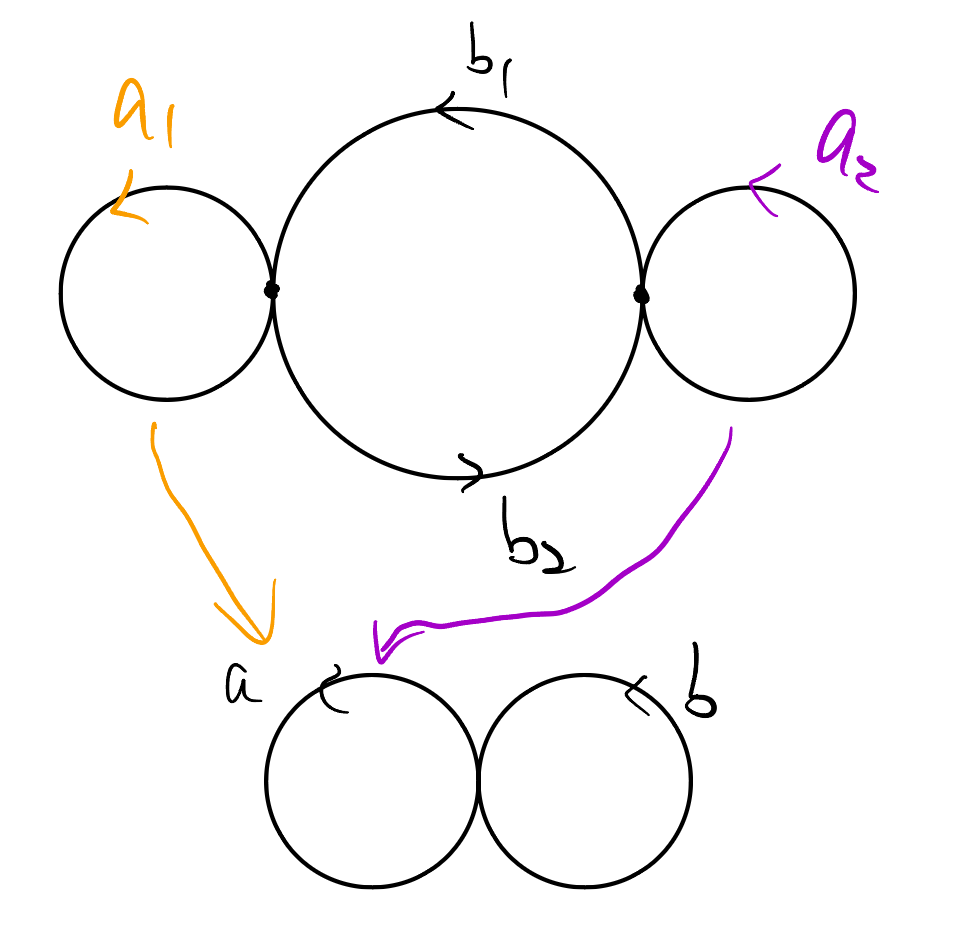
\includegraphics[width=0.4\textwidth]{./figures/2-cover-8.png}
	\caption{}
\end{figure}
Consider the 1-simplices $ a_1: \Delta_1 \to Y$ and $ a_2: \Delta_1 \to Y$. Since $ Y$ is 1-dimensional, the image of any 2-simplex must be at most 1-dimensional, and the boundary must be at most 0-dimensional. Thus $ a_1 - a_2$ is 1-dimensional and not a boundary of a 2-simplex, \emph{i.e.} they are distinct elements in the homology. However, since $ p \circ a_1 = a = p \circ a_2$, $ p_*([ a_1]) = [ a] = p_*([ a_2])$, showing that $ p_*$ is not injective.
\end{problem}
\begin{problem}[4]
Note that any possible pair is a good pair in this problem, since contractible implies that we can just treat the subspace as a point, and the subspace deformation retracts to the point via contractibility. Denote $ X_{12} := X_1 \cup X_2$. First I claim that $ H_n(X_{12}) = 0$ for $ n\geq 2$. If  $ X_2$ is empty then it is trivially true. If $ X_2$ is contractible, we have
\begin{align*}
	H_n(X_{12}) \cong \widetilde{ H}_n(X_{12}/X_2) \cong \widetilde{ H}_n(X_1 / (X_1 \cap X_2)) = \widetilde{ H}_n(*) = 0
\end{align*}
Next, I claim that $ H_n(X_{12} \cap X_3) = 0$ for $ n \geq 1$. Suppose $ (X_1 \cap X_3) \cap (X_2 \cap X_3) = X_1 \cap X_2 \cap X_3 = \O $. Then by additivity, $ H_n(X_{12} \cap X_3) = H_n(X_1 \cap X_3) \oplus  H_n(X_2 \cap X_3) = 0 \oplus 0 = 0$. Suppose the three-way intersection is not empty, WLOG we can assume both two-way intersections are contractible (if they are empty we can use additivity again to get trivial homology), by Mayer-Vietoris on the two-way intersections in the obvious way we obtain $ H_n(X_{12} \cap X_3) = 0 $.

Finally, by Mayer-Vietoris, for $ n \geq 2$ we have
\begin{align*}
	H_n(X_{12} \cap X_3)=0 \to H_n(X_{12}) \oplus H_n(X_3) = 0 \to H_n(X) \to H_{n-1}(X_{12} \cap X_3) = 0
\end{align*}
So $ H_n(X) =0$.
\end{problem}

\begin{problem}[8]
Recall that a cone is contractible via the straight-line homotopy to the cone tip. Denote the top cone $ C_+(X)$ and bottom cone  $ C_-(X)$. Let  $ U_+$ be the top cone with some ``open skirt" and $ U_-$ be the bottom cone with open skirt. They union to  $ SX$ and deformation retract to their respective cone.
~\begin{figure}[H]
	\centering
	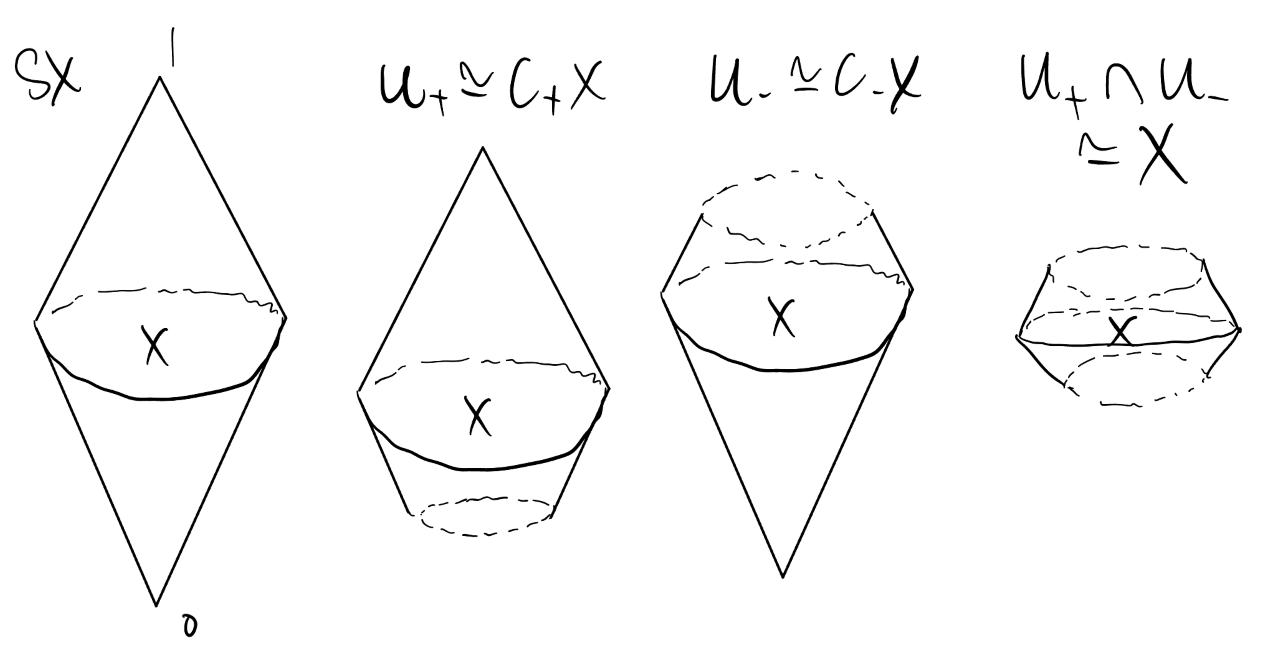
\includegraphics[width=0.8\textwidth]{./figures/MV_suspension.png}
\end{figure}

Thus $ H_n(C_{\pm}X) \cong H_n(U_{\pm}) = 0$ for $ n \geq 1$ and  $ \zz$ for $ n=0$. Moreover,  $ U_+ \cap U_- \simeq X$ so $ H_n(U_+ \cap U_-) \cong H_n(X)$. Now apply Mayer-Vietoris for $ n \geq 1$:
\begin{align*}
	\to \underbrace{ H_{n+1}(U_+) \oplus H_{n+1}(U_-)}_{ 0} \to H_{n+1}(SX) \to \underbrace{ H_n(U_+ \cap U_-) }_{ \cong H_n(X)} \to \underbrace{ H_n(U_+) \oplus H_n(U_-)}_{ 0} \to
\end{align*}
So $ H_{n+1}(SX) \cong H_n(X)$ for $ n \geq 1$, and the reduced homology coincide with homology for this range. Outside this range, we have
\begin{align*}
	\to \underbrace{ H_{1}(U_+) \oplus H_{1}(U_-)}_{ 0} \to H_{1}(SX) \xrightarrow{ \partial }  \underbrace{ H_0(U_+ \cap U_-) }_{ \cong H_0(X)} \xrightarrow{ \phi}  \underbrace{ H_0(U_+) \oplus H_0(U_-)}_{ \zz \oplus \zz} \xrightarrow{ \psi}  \underbrace{ H_0(SX)}_{ \cong \zz}\to 0
\end{align*}
Since $ \psi$ is surjective, exactness and 1st isomorphism theorem yield $ \zz^2 / \im \phi \cong \zz$. Since $ \zz$ is free, we have a split short exact sequence $ 0 \to \im \phi \to \zz^2 \to \zz \to 0$ and hence $ \im \phi \oplus \zz \cong \zz^2$. Thus $ H_0(X) / \ker \phi \cong \im \phi \cong \zz$. By the same argument, $ H_0(X) \cong \ker \phi \oplus \zz$ so $ \widetilde{ H}_0(X) \cong \ker \phi = \im \partial \cong H_1(SX) = \widetilde{ H}_1(SX)$ since $ \partial $ is injective.

Finally, since $ SX$ is path-connected (can always connect two points via the cone tip),  $ \widetilde{ H}_0(SX) = 0 = \widetilde{ H}_{-1}(X)$.
\end{problem}

\begin{problem}[9]
We already know that $ T^2 := S^{1} \times S^{1}$ have
\begin{align*}
	H_n(T^2) &= \begin{cases}
		\zz^2 & n =2\\
		\zz & n=0,1\\
	\end{cases} \\
\end{align*}
Denote $ X = S^{1} \vee S^{1} \vee S^{2}$. Let $ A$ and  $ B$ be as shown in the figure. Clearly  $ A \simeq S^2$, $ B \simeq S^{1} \vee S^{1}$, $ A \cap B$ is contractible.
~\begin{figure}[H]
	\centering
	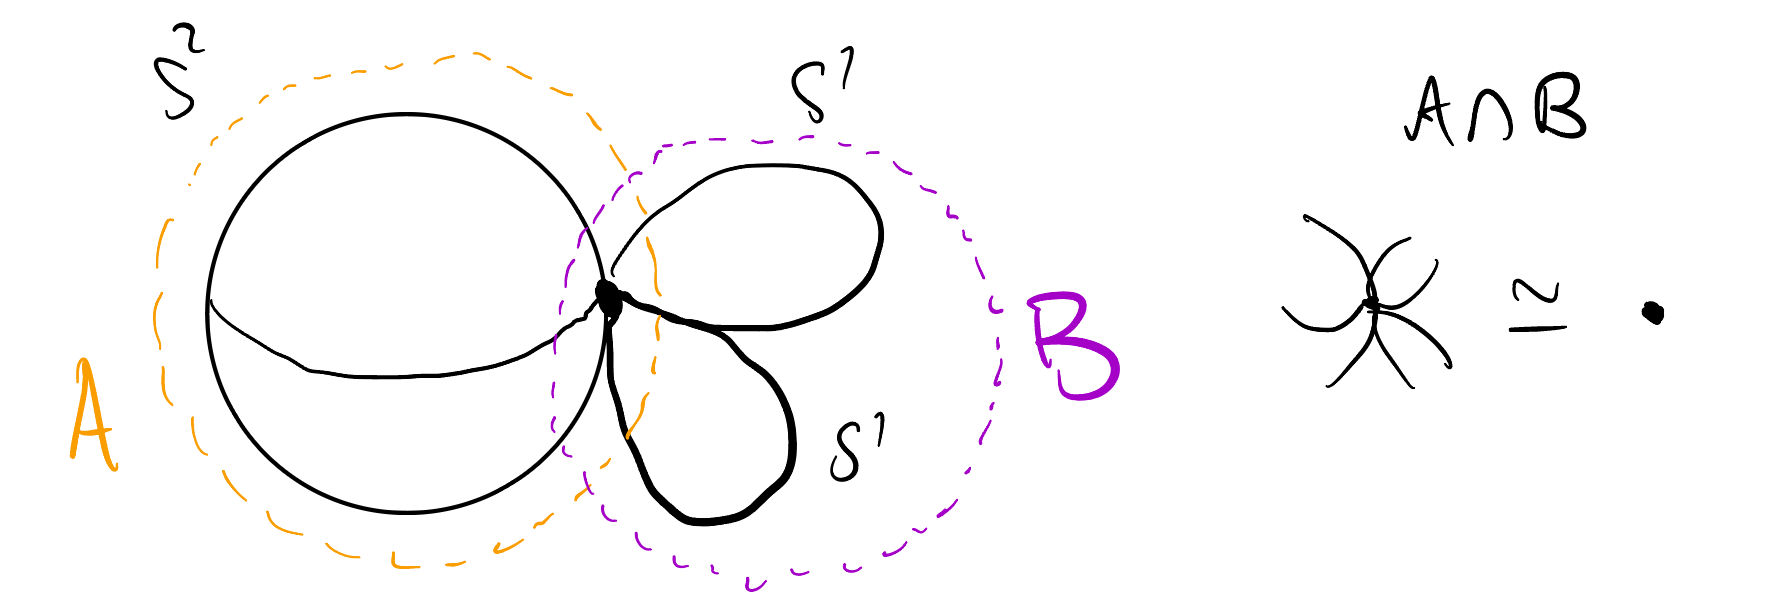
\includegraphics[width=0.8\textwidth]{./figures/MV_wedge.png}
\end{figure}
For $ i>2$, we have
\begin{align*}
	\cdots \to \underbrace{ H_i(A \cap B)}_{0 }  \to \underbrace{ H_i(A) \oplus H_i(B) }_{ 0 \oplus 0} \to H_i(X) \to \underbrace{ H_{i-1}(A \cap B)}_{ 0}  \to \cdots
\end{align*}
which implies $ H_i(X) = 0$. Else,
\begin{align*}
	\underbrace{ H_2(A \cap B)}_{ 0} \xrightarrow{ \phi_2}  \underbrace{ H_2(A) \oplus H_2(B)}_{ \cong \zz \oplus 0} \xrightarrow{ \psi_2}  H_2(X) \xrightarrow{ \partial_2}  \underbrace{ H_1(A \cap B)}_{ 0} \xrightarrow{ \phi_1}  \underbrace{ H_1(A) \oplus H_1(B)}_{ 0 \oplus \zz^2} \xrightarrow{ \psi_2}  H_1(X) \xrightarrow{ \partial _1}\\  
	\underbrace{ H_0(A \cap B)}_{ \cong \zz} \xrightarrow{ \phi_0} \underbrace{ H_0(A) \oplus H_0(B)}_{ \zz \oplus \zz} \to \cdots   
\end{align*}
We immediately have $ H_2(X) \cong H_2(A)\oplus H_2(B) \cong \zz$. Moreover, $ \psi_1$ is injective so $ \zz^2 \cong \im \psi_1 = \ker \partial _1 $. We see that $ \phi_0:1 \mapsto (1,1)$ is also injective, so $ \im \partial _1 = \ker \phi_0 = 0$, therefore by first isomorphism theorem, $ 0 = \im \partial _1 \cong H_1(X) / \ker \partial _1 =  H_1(X) / \zz^2$ which implies that $ H_1(X) = \zz^2$. Finally, $ X$ is clearly path-connected so  $ H_0(X) \cong \zz$. Therefore, the homology of $ X$ coincides with  $ T^2$. However, the universal cover of $ T^2$ is $ \rr^2$ which is contractible, yet the universal cover of $ X$ is the Caley tree of  $ F_2$ where each vertex wedges a $ S^2$, so it is homotopy equivalent to an infinity wedge of circles $ \bigvee^{ \infty} S^2$ by quotienting out the contractible Caley tree. Notice that we can apply Mayer-Vietoris on $ \bigvee^ \infty S^2 $ by letting $ A $ bean open set containing exactly one sphere, and  $ B$ be an open set containing the rest. Clearly  $ A \cap B$ is contractible, so it yields
\begin{align*}
	0 \to H_2(A) \oplus H_2(B) \to H_2(\bigvee^ \infty S^2) \to 0  
\end{align*}
That is, $H_2(\bigvee^ \infty S^2 ) \cong \zz \oplus H_2(B)$ which is not trivial. Since $ H_2(\rr^2) = 0$ yet $ H_2(\bigvee^{ \infty}S^2) \neq 0$, we prove the statement.
\end{problem}

\begin{problem}[10]
We think of $ \rr P^2$ as a disk with antipodal points in the boundary identified. Let $ A,B$ be as shown in the figure below.
~\begin{figure}[H]
	\centering
	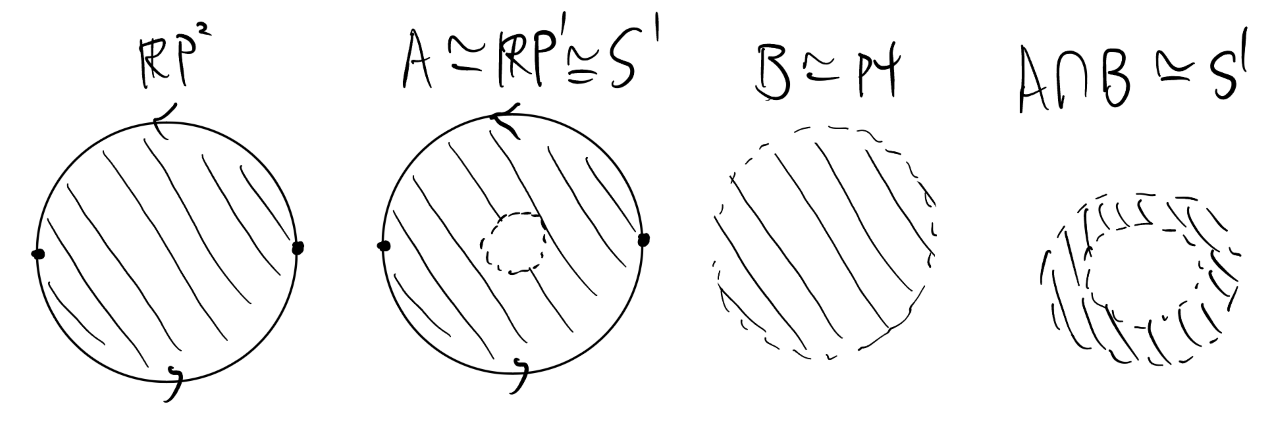
\includegraphics[width=0.8\textwidth]{./figures/MV_RP2.png}
	\caption{}
\end{figure}
We see that $ B$ is an open disk which is contractible, and $ A \cap B$ is an open annulus which is homotopy equivalent to $ S^{1}$. Finally, we see that by deformation retracting to the boundary, $ A$ is homotopy equivalent to a circle with antipodal points identified, which is exactly $ \rr P^{1}$. It is easy to see that for $i>2 $, all parts involved have zero homology so $ H_i( \rr P^2) = 0$ for this range. Consider,
\begin{align*}
	\cdots \to \underbrace{ H_2(A) \oplus  H_2(B)}_{ 0 \oplus 0}  \xrightarrow{ \psi_2} H_2 (\rr P^2) \xrightarrow{ \partial_2} \underbrace{ H_1(A \cap B)}_{ \langle f_1-f_2 \rangle \cong \zz} \xrightarrow{ \phi_1} \underbrace{ H_1(A) \oplus H_1(B)}_{\langle g_1- g_2 \rangle \cong\zz \oplus 0} \xrightarrow{ \psi_1} H_1(\rr P^2) \xrightarrow{ \partial _1}\\
	\underbrace{ H_0(A \cap B)}_{ \cong \zz } \xrightarrow{ \phi_0} \underbrace{ H_0(A) \oplus H_0(B)}_{ \cong \zz\oplus \zz } \to \cdots    
\end{align*}
By figure, we see that inlusion of $ f_1-f_2$ into $ A$ wraps around the generator  $ g_1-g_2$ twice due to the identification. Hence $ \phi_1$ indices multiplication by 2 on the homology. Hence $ 0=\ker \phi_1 = \im \partial _2  = H_2(\rr P^2)$ and $ \im \phi_1 = 2 \zz$. Since $ \phi_0: 1 \mapsto (1,1)$ is injective, $ \im \partial _1 = \ker \phi_0 =0$. Thus $ \psi_1 $ is surjective and $ H_1(\rr P^2) = \im \psi_1 = \zz / \ker \psi_1 \cong \zz / \im  \phi_1 = \zz / 2 \zz =  \zz /2$.

In summary, we have
\begin{align*}
	H_i (\rr P^2) = \begin{cases}
		0 & i > 1\\
		\zz /2 & i =1\\
		\zz & i = 0\\
	\end{cases}.
\end{align*}

For $ \rr P^3$, let $ A,B$ be analogous open set on $ D^3$ with boundary antipodal points identified. Then $ A \simeq \rr P^2$, $ B \simeq \text{*}$, and $ A \cap B \simeq S^2$. Again for $ i>3$,  $ H_i(\rr P^3) =0$. Consider
\begin{align*}
	\cdots \to \underbrace{ H_3(A) \oplus  H_3(B)}_{ 0 \oplus 0}  \xrightarrow{ \psi_3} H_3 (\rr P^3) \xrightarrow{ \partial_3} \underbrace{ H_1(A \cap B)}_{ \cong \zz} \xrightarrow{ \phi_2} \underbrace{ H_2(A) \oplus H_2(B)}_{0\oplus 0} \xrightarrow{ \psi_2} H_2(\rr P^3) \xrightarrow{ \partial _2}\\
	\underbrace{ H_1(A \cap B)}_{0} \xrightarrow{ \phi_1} \underbrace{ H_1(A) \oplus H_1(B)}_{\zz /2 \oplus 0 } \xrightarrow{ \psi_1} H_1(\rr P^3) \xrightarrow{ \partial_1}  \underbrace{ H_0(A \cap B)}_{ \cong \zz } \xrightarrow{ \phi_0} \underbrace{ H_0(A) \oplus H_0(B)}_{ \cong \zz\oplus \zz } \to \cdots    
\end{align*}

We immediately have $ H_3(\rr P^3) \cong \zz$. By the same argument as in $ \rr P^2$, $ \partial _1$ is surjective, so $ H_1(\rr P^3) \cong  \zz /2 / \ker \psi_1 \cong \zz /2$.

In summary, we have
\begin{align*}
	H_i (\rr P^3) = \begin{cases}
		0 & i > 3\\
		\zz /2 & i =1\\
		\zz & i = 0,3\\
	\end{cases}.
\end{align*}


\end{problem}
\end{document}
